\documentclass{fkssolpub}

\usepackage[czech]{babel}
\usepackage{fontspec}
\usepackage{fkssugar}
\usepackage{amsmath}
\usepackage{graphicx}

\author{Ondřej Sedláček}
\school{Gymnázium Oty Pavla} 
\series{1}
\problem{3} 

\begin{document}

\begin{figure}[h!]
	\begin{center}
		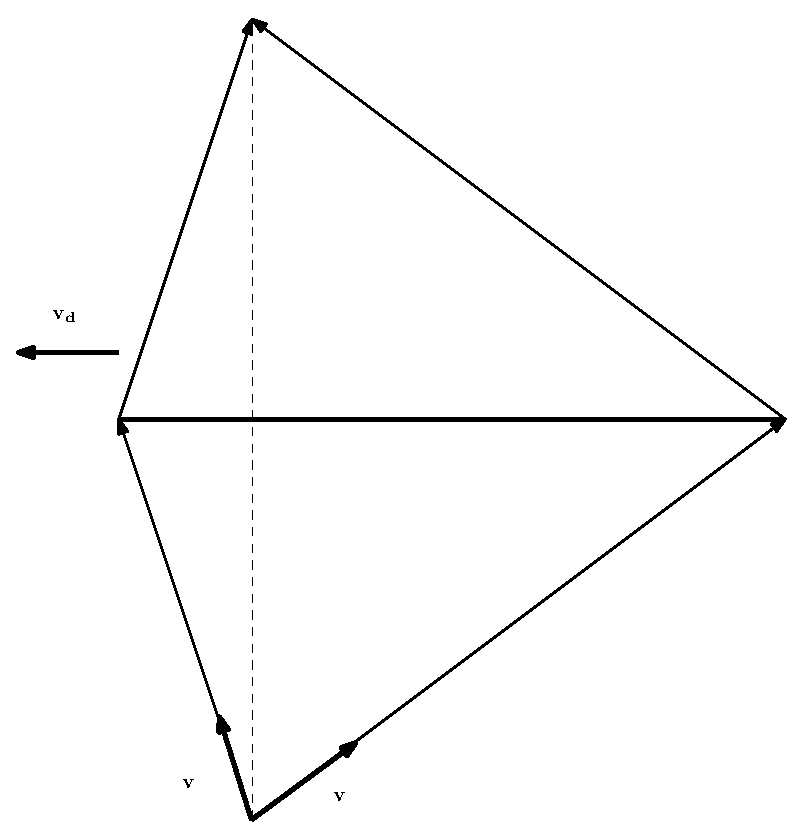
\includegraphics[width=0.5\textwidth]{3-fig.eps}
	\end{center}
	\caption{Náčrt situace}
	\label{fig:1}
\end{figure}

Jarda má na výběr dvě možnosti -- buď zástup oběhne zepředu, nebo zezadu. Z náčrtu výše vidíme, že délku obou tras umíme spočítat s použitím Pythagorovi věty:

\[
	s_1 = 2 \cdot \sqrt{25^2 + \left(v_d \cdot \frac{t_1}{2}\right)^2}
\]
\[
	s_2 = 2 \cdot \sqrt{25^2 + \left(10 - v_d \cdot \frac{t_2}{2}\right)^2}
\]

A protože obě trasy půjde konstantní rychlostí získáme dvě rovnice, které potřebujeme vyřešit:

\[
	v t_1 = 2 \cdot \sqrt{25^2 + \left(v_d \cdot \frac{t_1}{2}\right)^2}
\]
\[
	v^2 t_1^2 = 4 \cdot 25^2 + v_d^2 t_1^2
\]
\[
	(v^2 - v_d^2) t_1^2 = 50^2
\]
\[
	t_1 = \frac{50}{\sqrt{v^2 - v_d^2}} \doteq "35{,}36 s"
\]

\[
	v t_2 = 2 \cdot \sqrt{25^2 + \left(10 - v_d \cdot \frac{t_2}{2}\right)^2}
\]
\[
	v^2 t_2^2 = 50^2 + 400 - 40v_d t_2 + v_d^2 t_2^2
\]
\[
	(v^2 - v_d^2) t_2^2 + 40 v_d t_2 - (400 + 50^2) = 0
\]
\[
	t_2 \doteq "33{,}406 s"
\]

Protože obě rovnice mají jen jediné kladné řešení, výsledky jsou $t_1 \doteq 35{,}36 "s"$ a $t_2 \doteq 33{,}406 "s"$, tedy oběhnutí zástupu zezadu je rychlejší. Ještě si ale zkontrolujeme, zda už zástup nestihne uhnout ze spojnice:

\[
	33{,}406 \div 2 \cdot "0{,}5 m" \doteq "8.35 m" < "10 m"
\]

Protože zástup ze spojnice nestihne uhnout, nejkratší čas je tedy 33{,}406 s.





\end{document}
